\chapter{Introduction}


\section{Background}

This thesis was written between late 2021 and early 2025, a period marked by unprecedented advances in generative artificial intelligence (AI). Driven by innovations in deep neural networks \cite{Goodfellow-et-al-2014}, enhanced computational capabilities through graphical processing units (GPUs) \cite{Dean-et-al-2012}, and access to extensive training datasets \cite{Deng-et-al-2009}, AI systems have evolved from producing basic outputs to generating sophisticated content across multiple domains.

The progression in image generation has seen models advance from basic figure generation to creating photorealistic images and diverse artistic styles through natural language prompts \cite{Ramesh-et-al-2022}. Language models, which previously struggled with coherent text generation beyond brief passages prior to 2021, now demonstrate capabilities in extended narrative composition, complex problem-solving—occasionally surpassing PhD-level expertise—code generation, tool utilization, and computer control \cite{Brown-et-al-2020}. Similar advances have emerged in music generation, progressing from simple melodic sequences to full musical compositions \cite{Huang-et-al-2020}, while significant developments have occurred in video generation \cite{Sohn-et-al-2015}. In scientific applications, generative algorithms have achieved remarkable breakthroughs, notably in protein structure prediction, leading to Nobel Prize recognition for AI researchers \cite{NobelPrize2024}.

The commercial deployment of ChatGPT in November 2022 represented a pivotal moment, achieving unprecedented user adoption rates. Subsequently, comparable systems such as Gemini and Claude have emerged, alongside image generation platforms including MidJourney, Leonardo, and Stable Diffusion, collectively attracting millions of users across diverse applications. These generative technologies serve multiple user demographics: educators developing curricula, students composing academic work, language learners practicing writing, information seekers, fiction authors, researchers conducting studies, professionals crafting correspondence, designers prototyping concepts, visual artists creating artwork, and musicians composing personalized pieces.

Recent years have witnessed the mainstream integration of generative AI, characterized by expanding capabilities and adoption rates that suggest profound implications for various aspects of human activity.

Within the broader discourse surrounding artificial intelligence—encompassing ethical, social, economic, and political dimensions—a fundamental question emerges regarding its interaction with human creativity. The potential for AI to augment, transform, or potentially supersede human creative endeavors remains an active area of academic investigation \cite{Boden-2004, Runco-Jaeger-2012}.

This thesis examines the potential for human-AI co-creativity, specifically investigating the design principles for AI systems that can function as effective co-creators with humans, facilitating synergistic integration between machine-generated and human creativity.
 
\section{Human-AI Co-Creativity}

Historically, new technologies and human creativity have co-evolved in complex ways, bringing new possibilities as well as challenges. An illustrative example is the development of the camera, which prompted extensive discussion in the 20th century regarding its impact on art and its value as a creative medium. The French poet Charles Baudelaire claimed that "photography is the refuge of ill-endowed painters" and argued that it would be the death of French artistic genius \cite{Baudelaire-1955}. Critics such as Walter Benjamin discussed the alienating effects of the mechanization of visual production \cite{Benjamin-1935}. Indeed, some creative practices, such as portraiture, were replaced by photography. Painters like René Magritte initially made a living by creating illustrations for magazine covers and commercial materials, a niche eventually supplanted by photographic content.

Conversely, today, photography is recognized as a rich creative practice in its own right and has significantly expanded the creative possibilities in visual art, as extensively discussed by Aaron Scharf \cite{Scharf-1968}. Moreover, many artists and critics have noted the influence of photography on the development of new painting styles, such as Impressionism \cite{Sontag-1978}. Vincent van Gogh remarked, "It is the advantage that Impressionism possesses over all the other things; it is not banal, and one seeks after a deeper resemblance than the photographer's." The development of Impressionism can be partly understood as a response to photography's ability to capture the world realistically, thus crafting a new niche within creative ecologies.

Broadly, we can say that technologies can either replace creative work, such as the camera replacing portraiture and magazine illustrations; outsource aspects of the creative process, as when writers use spellcheckers or word processors instead of handwriting; or support creative endeavors, exemplified by design systems like Photoshop. Within this categorization, AI introduces the possibility of a fourth scenario: co-creativity, where the machine exhibits creative behavior that interacts synergistically with human creativity. 

Scholars have increasingly argued that generative AI systems can—and perhaps should—be seen as more than mere tools. Instead, they may function as co-creators capable of reciprocally shaping creative processes \cite{Davis2013-jy, Rezwana2023-rt, Wan2023-he, McCormack2008-rs, Lawton2023-tb, Bown2020-zn, Moruzzi2024-cq}. Empirical findings support the idea that such collaborations can enhance overall creativity and produce superior results compared to either agent operating alone \cite{Jia2024-vp, Hitsuwari2023-tw, Vaccaro2024-ne}. Moreover, studies have shown that AI systems can broaden artistic and design possibilities, opening new avenues for exploration in both professional and personal creative endeavors \cite{Bown2018-op, Ocampo2024-dv, Park2024-gw, Palani2024-on, Oh2018-mu}.

Despite their promise, current generative AI systems still exhibit notable constraints paticularly at the interface and interaction layer. They are sometimes opaque, difficult to steer, and insufficiently responsive to the evolving goals of a creative project \cite{Moruzzi2024-cq, El-Assady2022-qc}. Many systems retain only minimal context or rely heavily on a “command-and-control” style of interaction, wherein users issue prompts or directives to an AI treated primarily as a subservient tool. Such frameworks can be ill-suited for the nuanced dynamics of creativity, which often unfold through fluid iteration, reflection, and collaborative feedback loops \cite{Guzik2023-cl, Bown2021-os, Alexander2024-pz, Haase2023-vz}.

While most of the progress in the field of generative AI has happened at the model and algorithmic level, equally important is research in the interaction design layer \cite{Lin2023-zq, Bown2021-os} that studies how these systems can succesfully engage with users. 

Talk about the background. Cite Caterina. 

Definition here. 

This begs the question: can machines be creative. 

3Ps, AUT, argue the case for machine creativity. 

Cite Wiggins (unbiased observer)

Cite Dartmouth. Cite Colton. 

Ok, so if machines can be creative how do enable it. 

What are the challenges (cite other people). 

Human: overrealiance, skill loss, critical thinking. 
AI: lack of control, random, difficulty sterring, black box algorithms, generic style, explainability. 
At the intersection: mutual understanding.

Hypothesis: 
Dialogic interaction. 
Modelling dialogue. 
HCI concept. 

Establish research questions here. 
Potential, etc

\section{Methodology}

Mixed methods. 
Interaction Design Research. 
Creative practice. 
Across language and writing. 
Image generation. 
New Media Creative and Interactive Installations. 

Show diagram. 

\subsection{Thesis structure}
Outline the experiments I did. 
Not in order. 

Chapter 3: establish dialogic interaciton. Serves as a lens. Contrbution of this chapter is an elaboration of dialogic interaction as an HCI concept. 
Chapter 4: describes two experiments in new media. Context. New creative possibilities of language models. 
Chapter  5: describes two case studies in image generation. 
Chapter 6: describes two experiments, one a public prototype called Narrative Device. Second, a prototype developed in two stages exploring shared spaces. 

\subsection{Unique Contribution
}
Dialogic Co-Creativity as an Human Computer Interaction Design Concept that can be used to guide the development and analyse of co-creative systems
Design Principles for Co-Creative Systems
Six dimensions of Co-Creative AI to be considered when designing co-creative AI. 

Among things that made it particularly unique: 
Creative led explorations, in the real world, engaging with real creative industries, users and applications, developing tools that interacted with people

Conducted throughout a period of rapid development, which allowed to experiment with different technologies and draw design principles. 






Creativity and its products are central to the human experience. Art, music, design, technology, science philosophy are largely what we consider makes us human. Each of these practices has a close relationship with technology, embedded in a self-reinforcing feedback loop. New tools open up new creative possibilities, and new resistances. 

In 1800's the daguerrotype and photography opened up new possibilities. However, at the same time, the french poet Charles Baudeliere claimed that photography was the refuge of ill endowned painters. Today photography is a creative practice on its own. 

At the writing of this thesis, a major technological development is underway that similarly poses to deeply impact human creativity. That of artificial intelligence, in particular, generative rtificial intelligence. I began my thesis in 2021, when language models were in their infancy, image generation systems were primitive. Today, language models have achieved human level performance at some tasks. Outperformed humans at some tasks. Produce content that is indistinguishable from that produced by humans. Image models produce photorealistic images hard to distinguish from photos. Art that is indistinguishable from that produced by humans. Video generation and music generation are in their infancy, but one can expect they will follow a similar progression. 



While it is reasonable to speculate that this technology may follow a similar progression as other new tools: a period of awe, overblown promise, discovery of possibilities and resistance until its eventual consolidation as a mature tool within a niche of  creative ecologies, it is undeniable this is a fundamentally different type of technology. No other tool has been able to exhibit autnomous creative behavior and produced content that could pass at one produce by humans. How will humans interact with this technology? Will it fundamntally expand creative possibility? Will it replace the need for human creativity? How can we design generative AI systems that are able to beneficially expand the potential of creative action rather than diminish it? 

This thesis is concerned with examining the potential of human-AI co-creativity, such that the creativity of these tools engages in synergy with humans in a human desirable way. 

I address it from two perspectives. Creative-led practice based research practice and interaction design. 

\section{Human-AI Co-Creativity}

This thesis focuses on realizing the potential of \emph{human--AI co-creativity}: a synergistic relationship between human and machine where both parties iteratively influence the direction and quality of creative outcomes. 

- The field has changed a lot
- My thesis was conducted from 2021 to 2025. Period of rapid change. This was a blessing and a curse. It helped elucidate and keep close track. 
- Algorithmic progress has been very steep. But less research has gone into interaction design. 
- Some people are doing it. Build upon that work. (brief lit review)
- As new algorithms have emerged, new roles.
- New design principles. 
- New creative possibilities. 
- New modes of interaction. 
- Its a fresh field. 

I address it from two perspectives. Creative-led practice based research practice and interaction design. 

\section{Research Questions}

The principal aim of this thesis is to provide frameworks and insights into how we can design AI systems that \emph{partner} with human creators in a synergistic and empowering manner, while preserving and enhancing human creativity. Three research questions guide this investigation:

\begin{enumerate}
    \item \textbf{What co-creative roles can be assumed by generative AI systems?} 
    \item \textbf{What is the potential of dialogue as an interaction design concept for understanding and designing effective human--AI co-creativity?}
    \item \textbf{What design principles can guide the development of effective co-creative systems?}
\end{enumerate}

To address these questions, I adopt a practice-based, exploratory research methodology, which integrates user-centered studies, experimental prototypes, and analyses of real-world creative workflows. The intersections of technical advances in AI, interaction design, and creativity theory inform this research.

\section{A Dialogic Lens}

To reconfigure human--AI interactions for co-creativity, this thesis proposes adopting a \emph{dialogic} interaction model. By “dialogue,” I refer to an engagement characterized by mutual influence, co-creation, and shared meaning-making, in contrast to subject--object interactions where information flows in one direction \cite{Freire1970-pa, Bohm1996-fo, Buber1923-us}. While dialogic principles have been explored in fields such as education, philosophy, and social sciences, the prevalent paradigm in human--computer interaction (HCI) remains strongly shaped by command-and-control interfaces. Positioning AI as an active participant in an evolving conversation may better reflect the iterative and context-sensitive nature of creative work, helping establish more robust forms of co-creativity.

This thesis examines how dialogic principles can be operationalized in HCI systems that incorporate generative AI. Building on prior mixed-initiative research that advocates more collaborative relationships between humans and machines, I propose a design perspective that focuses on enabling mutual adaptation, iterative back-and-forth, and shared responsibility in creative tasks.

\begin{figure}
    \centering
    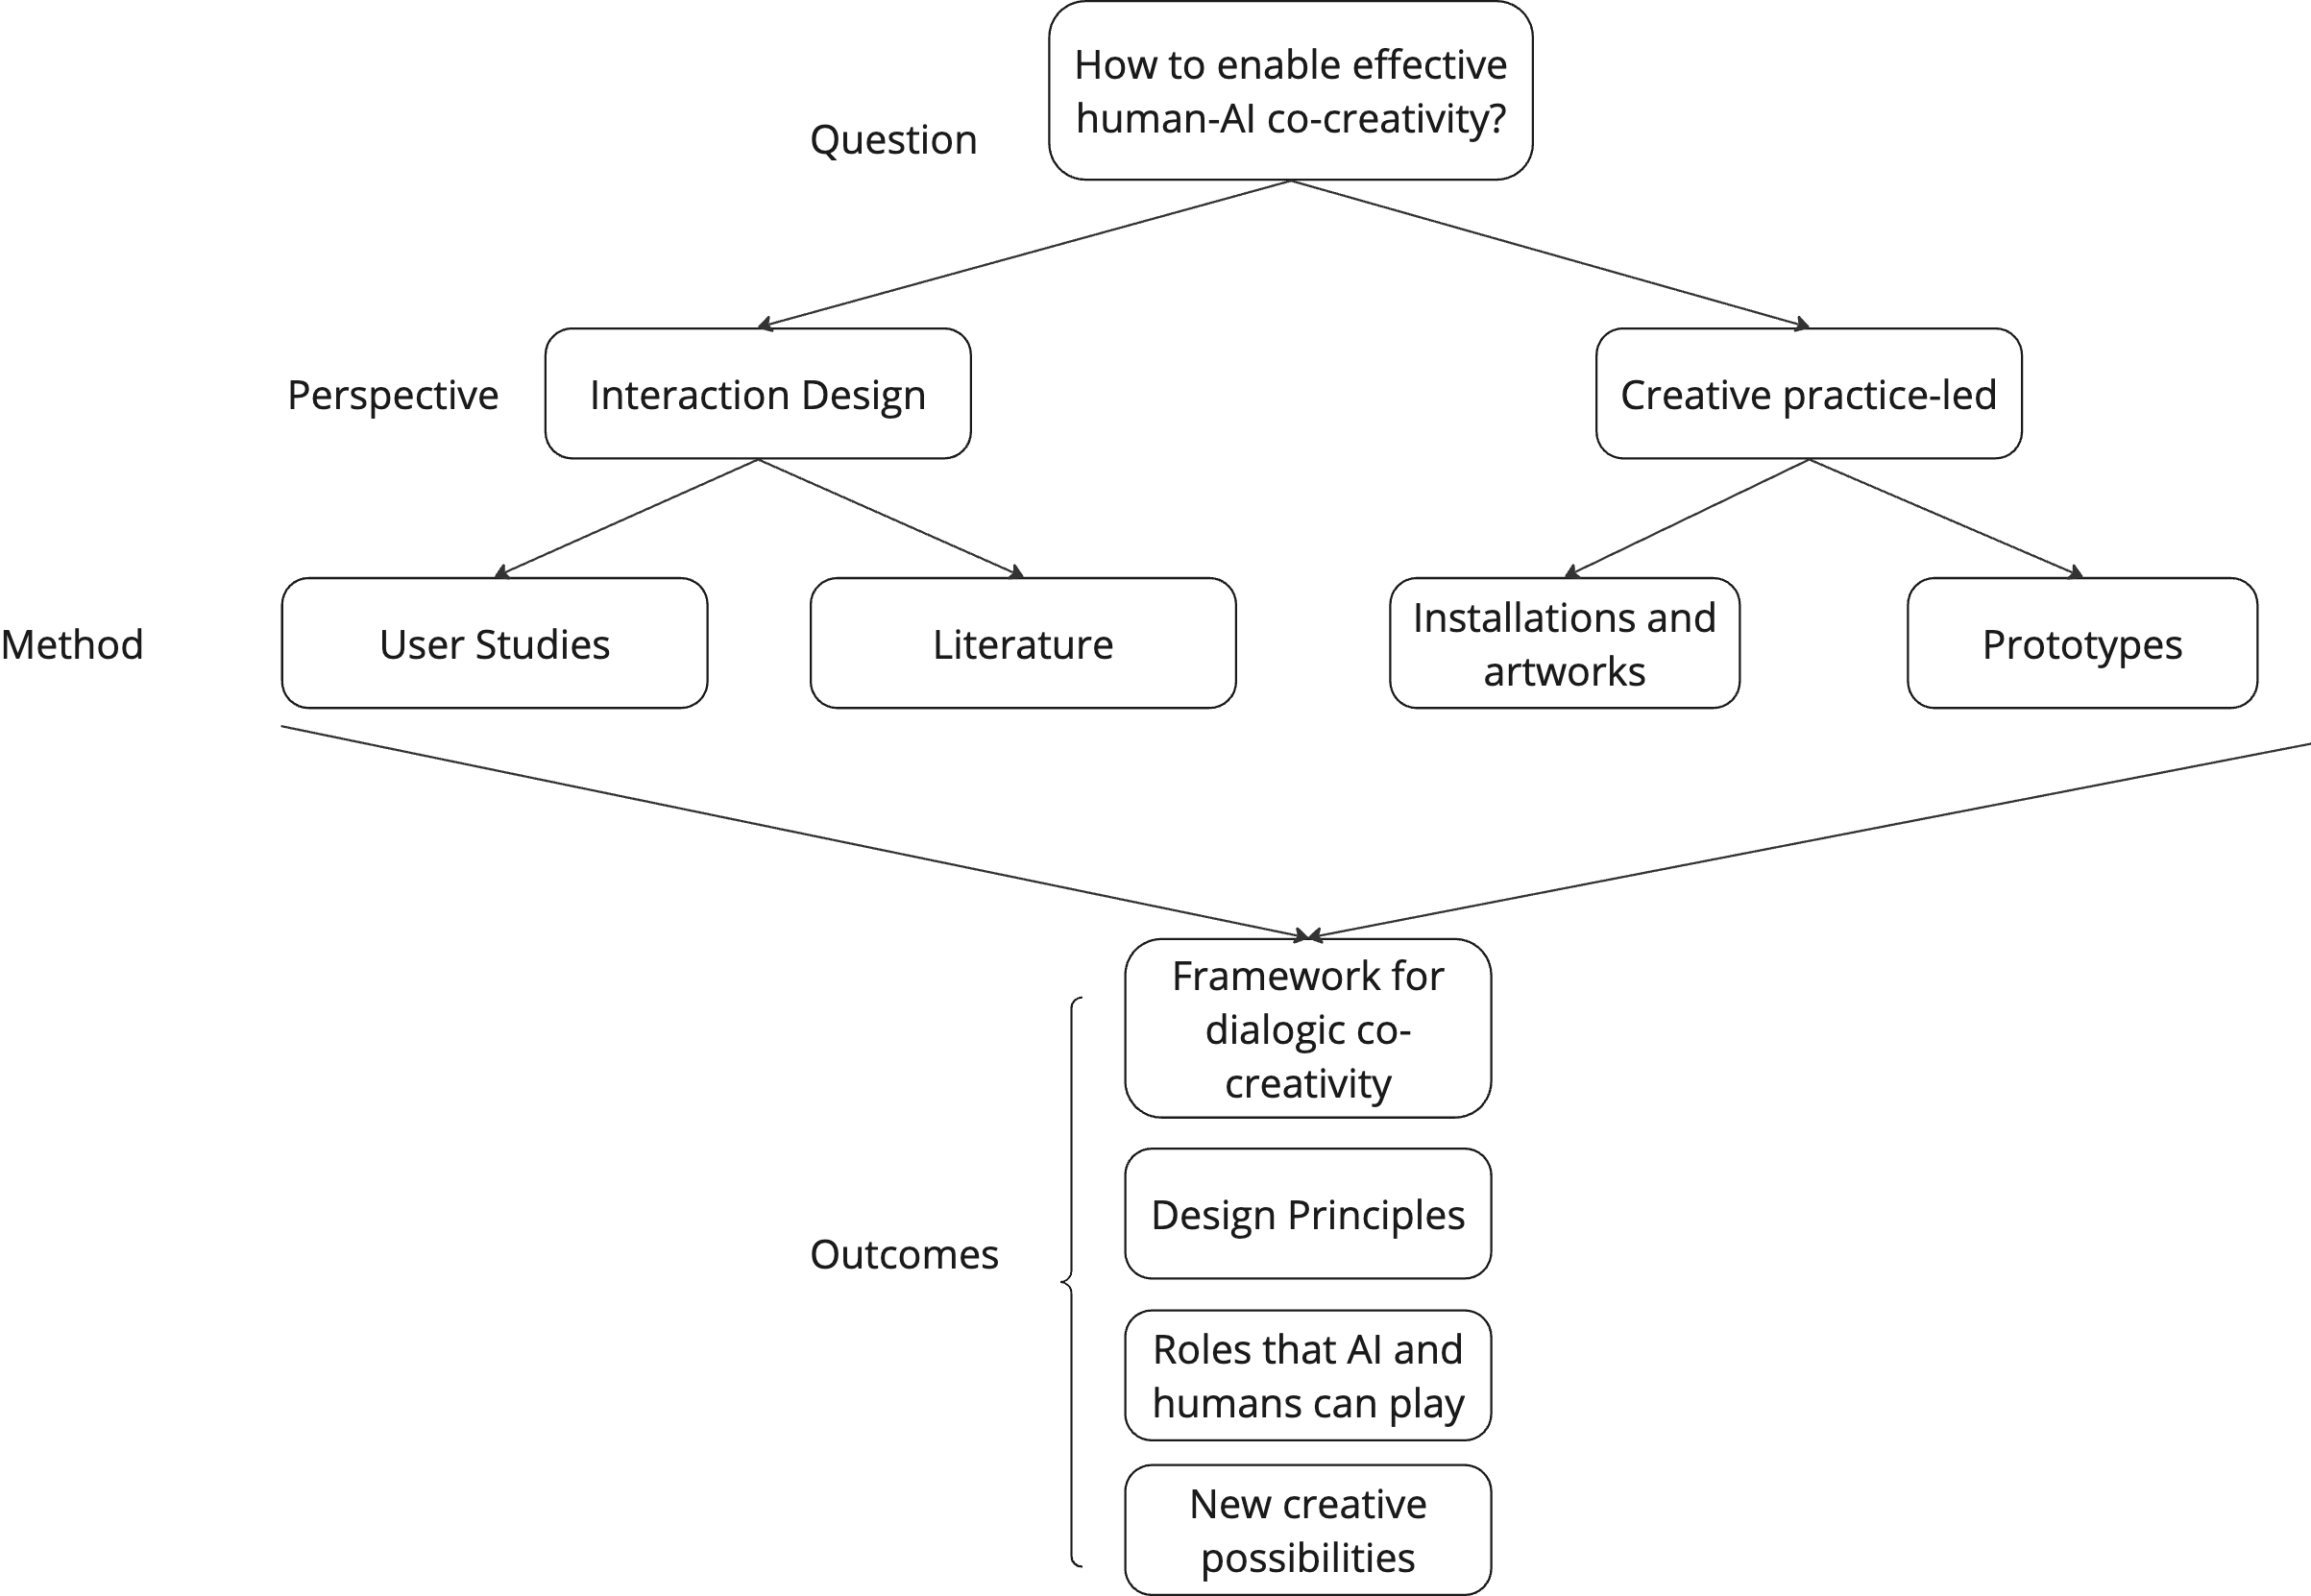
\includegraphics[width=0.75\linewidth]{researchstructure.png}
    \caption{Structure of how the core research question is addressed in this thesis}
    \label{fig:enter-label}
\end{figure}







